% Part: conditional-logics
% Chapter: minimal-change-semantics
% Section: true-false

\documentclass[../../../include/open-logic-section]{subfiles}

\begin{document}

\olfileid{con}{min}{tf}

\olsection{وجوه صدق الشرط المخالف وكذبه}

يصدق الشرط المخالف للواقع~$!A \cif !B$ صدقًا غير فارغ متى كانت
عوالم~$!A$ الأقرب كلها من عوالم~$!B$، كما يظهر في
\olref{fig:true}.
\begin{figure}
\begin{center}
\begin{tikzpicture}[scale=.7]\small
  \spheresystem{5}
  \draw (0,0) node {$\OLId{latin-ordinary}{w}$};
  \propositionintersect{0}{4}{40}{3.5}
  {\tikzset{proposition/.append={smooth,tension=1.4}}
  \proposition[shift={(1.6,-1)}]{90}{1}{30}{4}}
  \path (1.5,3) node[below] {$\formula{B}$};
  \path (3,0) node {$\formula{A}$};
\end{tikzpicture}
\caption{شرط مخالف للواقع صادق على نحو غير فارغ}
\ollabel{fig:true}
\end{center}
\end{figure}
ويصدق الشرط كذلك عند~$\OLId{latin-ordinary}{w}$ إذا خلا نظام الكرات المحيطة بـ$\OLId{latin-ordinary}{w}$ من كرة
تقبل~$!A$ أصلًا؛ وهذا هو الصدق \emph{على نحو فارغ}
(انظر~\olref{fig:vacuous}).
\begin{figure}
\begin{center}
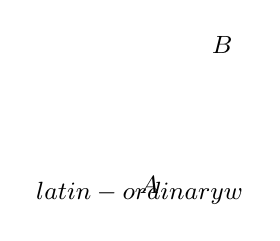
\begin{tikzpicture}[scale=.7]\small
  \spheresystem{5}
  \draw (0,0) node {$\OLId{latin-ordinary}{w}$};
  \proposition{0}{6.5}{40}{3.5}
  {\tikzset{proposition/.append={smooth,tension=1.4}}
  \proposition[shift={(1.2,-1)}]{90}{1}{30}{4}}
  \path (1.5,3) node[below] {$\formula{B}$};
  \spherepos{0}{7}{node {$\formula{A}$}}
\end{tikzpicture}
\caption{شرط مخالف للواقع صادق على نحو فارغ}
\ollabel{fig:vacuous}
\end{center}
\end{figure}

وللكذب صورتان. أولاهما أن يكون بعض أقرب عوالم~$!A$ من عوالم~$!B$
دون بعض؛ وعندئذ تكذب~$!A \cif \lnot !B$ أيضًا
(انظر~\olref{fig:false}).
\begin{figure}
\begin{center}
\begin{tikzpicture}[scale=.7]\small
  \spheresystem{5}
  \draw (0,0) node {$\OLId{latin-ordinary}{w}$};
  \propositionintersect{0}{4}{40}{3.5}
  {\tikzset{proposition/.append={smooth,tension=1.4}}
  \proposition[shift={(1.6,0)}]{90}{1}{30}{3}}
  \path (1.5,3) node[below] {$\formula{B}$};
  \path (3,0) node {$\formula{A}$};
\end{tikzpicture}
\caption{شرط مخالف للواقع كاذب، ومقابله كاذب}
\ollabel{fig:false}
\end{center}
\end{figure}
وأما إن لم يلتق أقرب عوالم~$!A$ بعوالم~$!B$ البتة، كذبت
$!A \cif !B$. وفي هذه الصورة تكون أقرب عوالم~$!A$ كلها عوالم
$\lnot !B$، فتصدق~$!A \cif \lnot !B$
(انظر~\olref{fig:false-opposite}).
\begin{figure}
\begin{center}
\begin{tikzpicture}[scale=.7]\small
  \spheresystem{5}
  \draw (0,0) node {$\OLId{latin-ordinary}{w}$};
  \propositionintersect{0}{4}{40}{3.5}
  {\tikzset{proposition/.append={smooth,tension=1.4}}
  \proposition[shift={(-1,0)}]{90}{1}{30}{3}}
  \path (-1,3) node[below] {$\formula{B}$};
  \path (3,0) node {$\formula{A}$};
\end{tikzpicture}
\caption{شرط مخالف للواقع كاذب، ومقابله صادق}
\ollabel{fig:false-opposite}
\end{center}
\end{figure}

وقد تكون الشرطيات المخالفة للواقع عرضية، بخلاف الشرط الصارم. ففي نموذج
الكرات في~\olref{fig:contingent} جميع عوالم~$!A$ الأقرب إلى~$\OLId{latin-ordinary}{u}$ من
عوالم~$!B$، ومن ثم~$\mSat{\OLId{latin-looped}{M}}{!A \cif !B}[\OLId{latin-ordinary}{u}]$. وأما بعض عوالم~$!A$
الأقرب إلى~$\OLId{latin-ordinary}{v}$ فليست من عوالم~$!B$، ومن ثم
$\mSat/{\OLId{latin-looped}{M}}{!A \cif !B}[\OLId{latin-ordinary}{v}]$.
\begin{figure}
\begin{center}
\begin{tikzpicture}[scale=.6]\small
  \spheresystem{7}
  \spheresystem[shift={(0:3.1)},dashed]{4}
  \propositionintersect{45}{4}{40}{4.5}
  \begin{scope}
    \clip \propositionplot{45}{4}{40}{4.5} ;
    \spherelayer[shift={(0:3.1)}]{3}
  \end{scope}
  \proposition[shift={(1.4,-.5)}]{90}{1}{35}{5}
  \path (0,0) node {$\OLId{latin-ordinary}{u}$};
  \path (0:3.1) node {$\OLId{latin-ordinary}{v}$};
  \spherepos{35}{9}{node {$\formula{A}$}}
  \spherepos{80}{9}{node {$\formula{B}$}}
\end{tikzpicture}
\end{center}
\caption{شرط مخالف للواقع عَرَضي}
\ollabel{fig:contingent}
\end{figure}
\end{document}



